\section{Using Cisco on AAU}
%husk at forklare om CPI og MSE
The Cisco localisation and positioning system is already in use at Aalborg University. To be able to use the information from the system, we had a meeting with the administrator, during which he raised concerns for privacy, as well as a desire of being able to provide this data to future student projects. To accommodate this, it has been asked of us to build and deploy an intermediate service with the goal of obfuscating sensitive personal data, such as mac-addresses and user names. This service is intended to duplicate the functionality of the Cisco Restful API, such that the service acts as a transparent proxy. This is achieved by creating an intermediate Restful service, that simply redirects requests and processes the response before sending it back to the initial requester, as illustrated on \cref{fig:cisco_usage}.

\begin{figure}[h]
	\begin{center}
	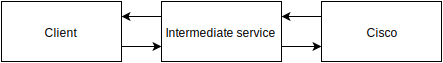
\includegraphics[scale=0.9]{graphics/cisco_usage.png}
	\caption{Cisco usage}
	\label{fig:cisco_usage}
	\end{center} 
\end{figure}

A Restful service typically communicates using the HTTP or HTTPS protocols, and functions by receiving requests on specific URIs to which it responds in a predefined fashion. As an example we can send a HTTPS GET request to 64.103.26.61 with the URI "/api/contextaware/v1/location/clients" and, given that we supply the correct user name and password, receive a string of data corresponding to the type of request. \sfx{relevant with example? We know that the given IP is a cisco test system, but should we use that in our report?} \sfx{kilde}

To create a transparent Restful service that duplicates the functionality of the Cisco Restful API, we need to make use of the same URIs as the Cisco API\sfx{link to cisco api}. This is done with the use of the Jersey Java library, which affords the possibility of creating a HTTP server and specifying what URIs are available for a client to request.

\begin{lstlisting}[caption={Adding a URI},label={lst:context_code},language=inc_Java]
server.createContext("/api/contextaware/v1/location/clients", httpExchange -> {
            if (VerifyConnection(httpExchange) == false){
                return;
            }

            String response = CollectAllClients(username, password, ciscoIp);
            httpExchange.sendResponseHeaders(200, response.length());
            OutputStream os = httpExchange.getResponseBody();
            os.write(response.getBytes(Charset.forName("UTF-8")));
            os.close();
        });
\end{lstlisting}
The code example shown on \cref{lst:context_code} shows an example of how to specify a URI. The createContext() method on line 1 takes two parameters: a string for the URI and an anonymous function implementing an interface. The anonymous function taking up the rest of the example dictates what actions are performed once a connection is established. In this case some verification is performed immediately after the function call, to authenticate the user. A response is generated based on the URI; on line 4 we retrieve all clients from Cisco using the ColletAllClients() function, which also performs the task of obfuscating necessary information. The list of clients is then written though an OutputStream to the requester, as seen on lines 8 and 9. The anonoymous function terminates as the OutputStream is closed, which also serves as a termination of the HTTP connection. 

In order to accommodate the privacy concern, we implement some simple methods to obfuscate mac-address and user name.  % TODO: show these methods